% !TeX root = ..\main.tex
\section{Thiết kế lược đồ BPMN}

Các lược đồ BPMN được nhóm thiết kế trên app Bizagi.
\subsection{Khách hàng mua hàng}
    \begin{figure}[!htp]
        \centering
        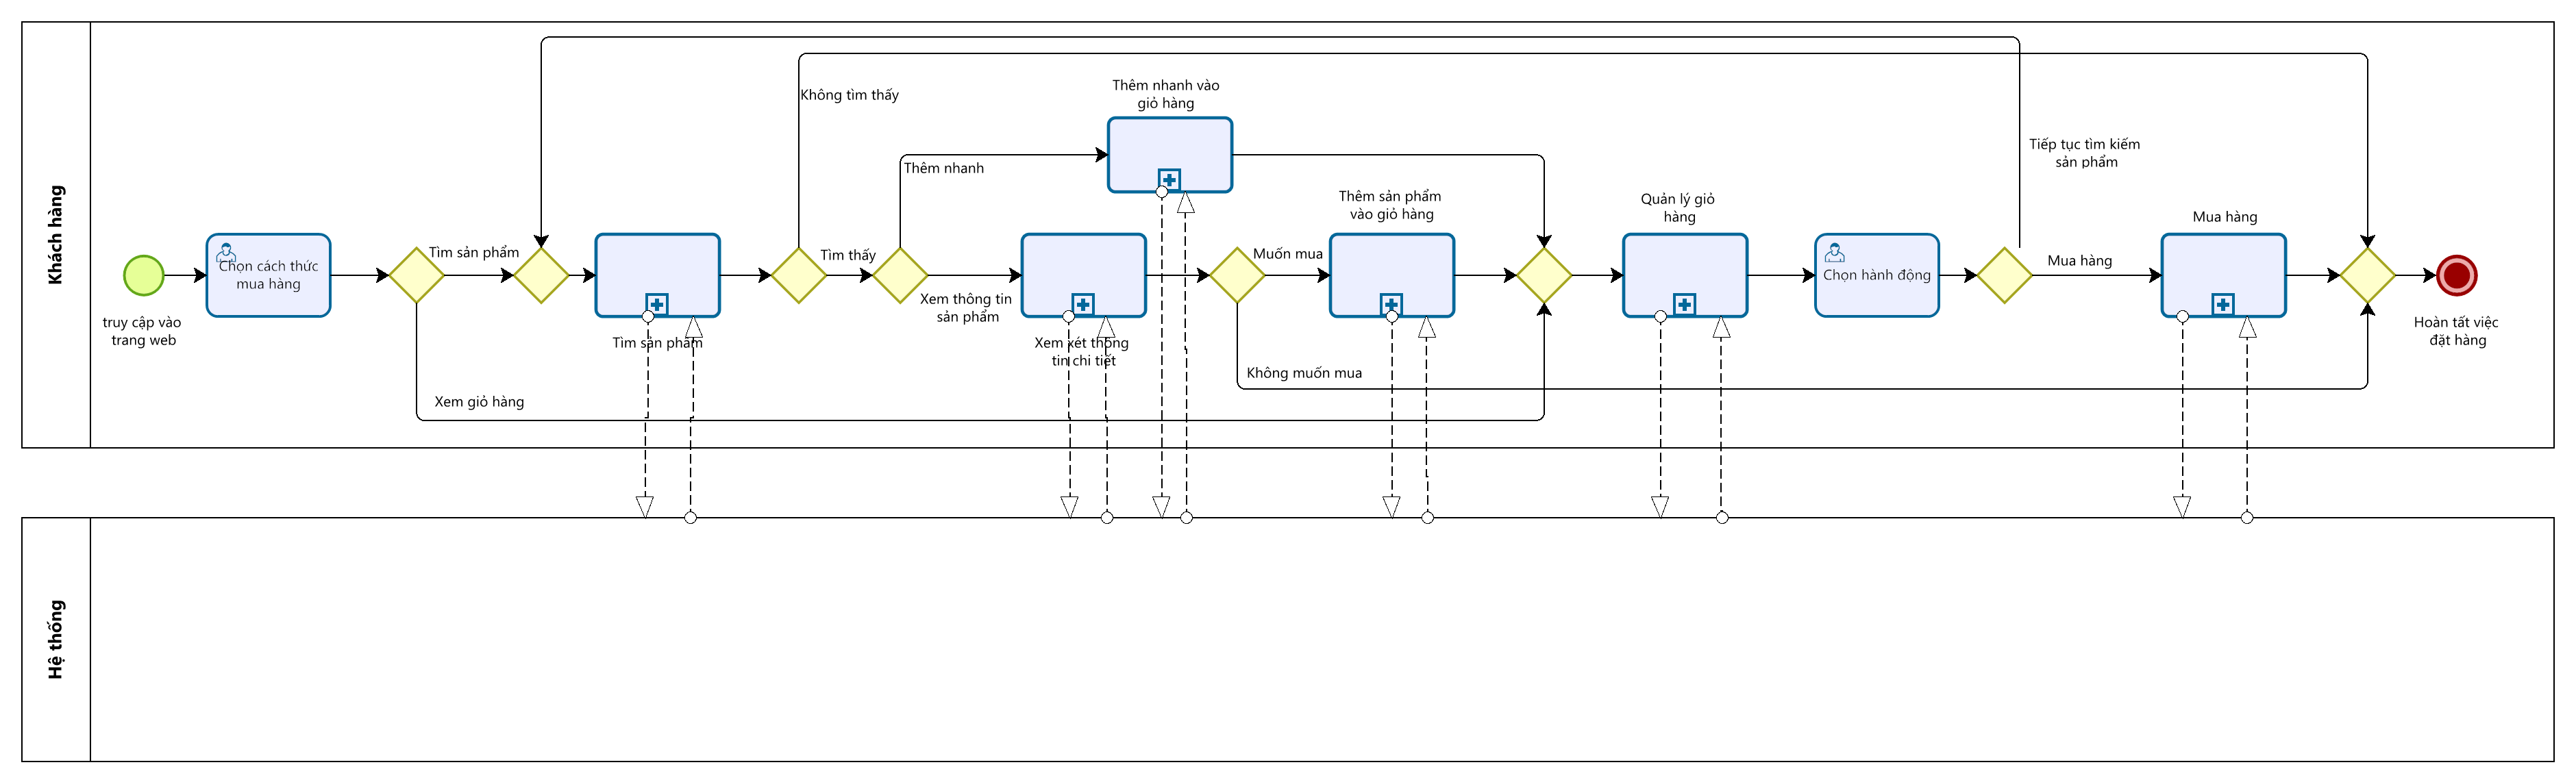
\includegraphics[width=17cm]{img/BPMN/customer_buy/customer_buy.png}
        \label{4}
        \newline
        \caption{Lược đồ BPMN cho quy trình khách hàng mua hàng}
    \end{figure}
    \textbf{Mô tả:}
    \begin{itemize}
        \item \textbf{Tìm sản phẩm}: Đây là 1 quy trình con chứa quy trình tìm kiếm sản phẩm của  khách hàng.
        \item \textbf{Xem xét thông tin chi tiết}: Đây là 1 quy trình con chứa quy trình xem thông tin chi tiết sản phẩm của  khách hàng.
        \item \textbf{Thêm sản phẩm vào giỏ hàng}: Đây là 1 quy trình con chứa quy trình thêm sản phẩm vào giỏ hàng.
        \item \textbf{Thêm nhanh vào giỏ hàng}: Đây là 1 quy trình con chứa quy trình thêm nhanh sản phẩm vào giỏ hàng.
        \item \textbf{Quản lý giỏ hàng}: Đây là 1 quy trình con chứa quy trình quản lý giỏ hàng của khách hàng.
        \item \textbf{Mua hàng}: Đây là 1 quy trình con chứa quy trình của việc mua hàng trong các giỏ hàng khách hàng.
    \end{itemize}
    \begin{figure}[!htp]
        \centering
        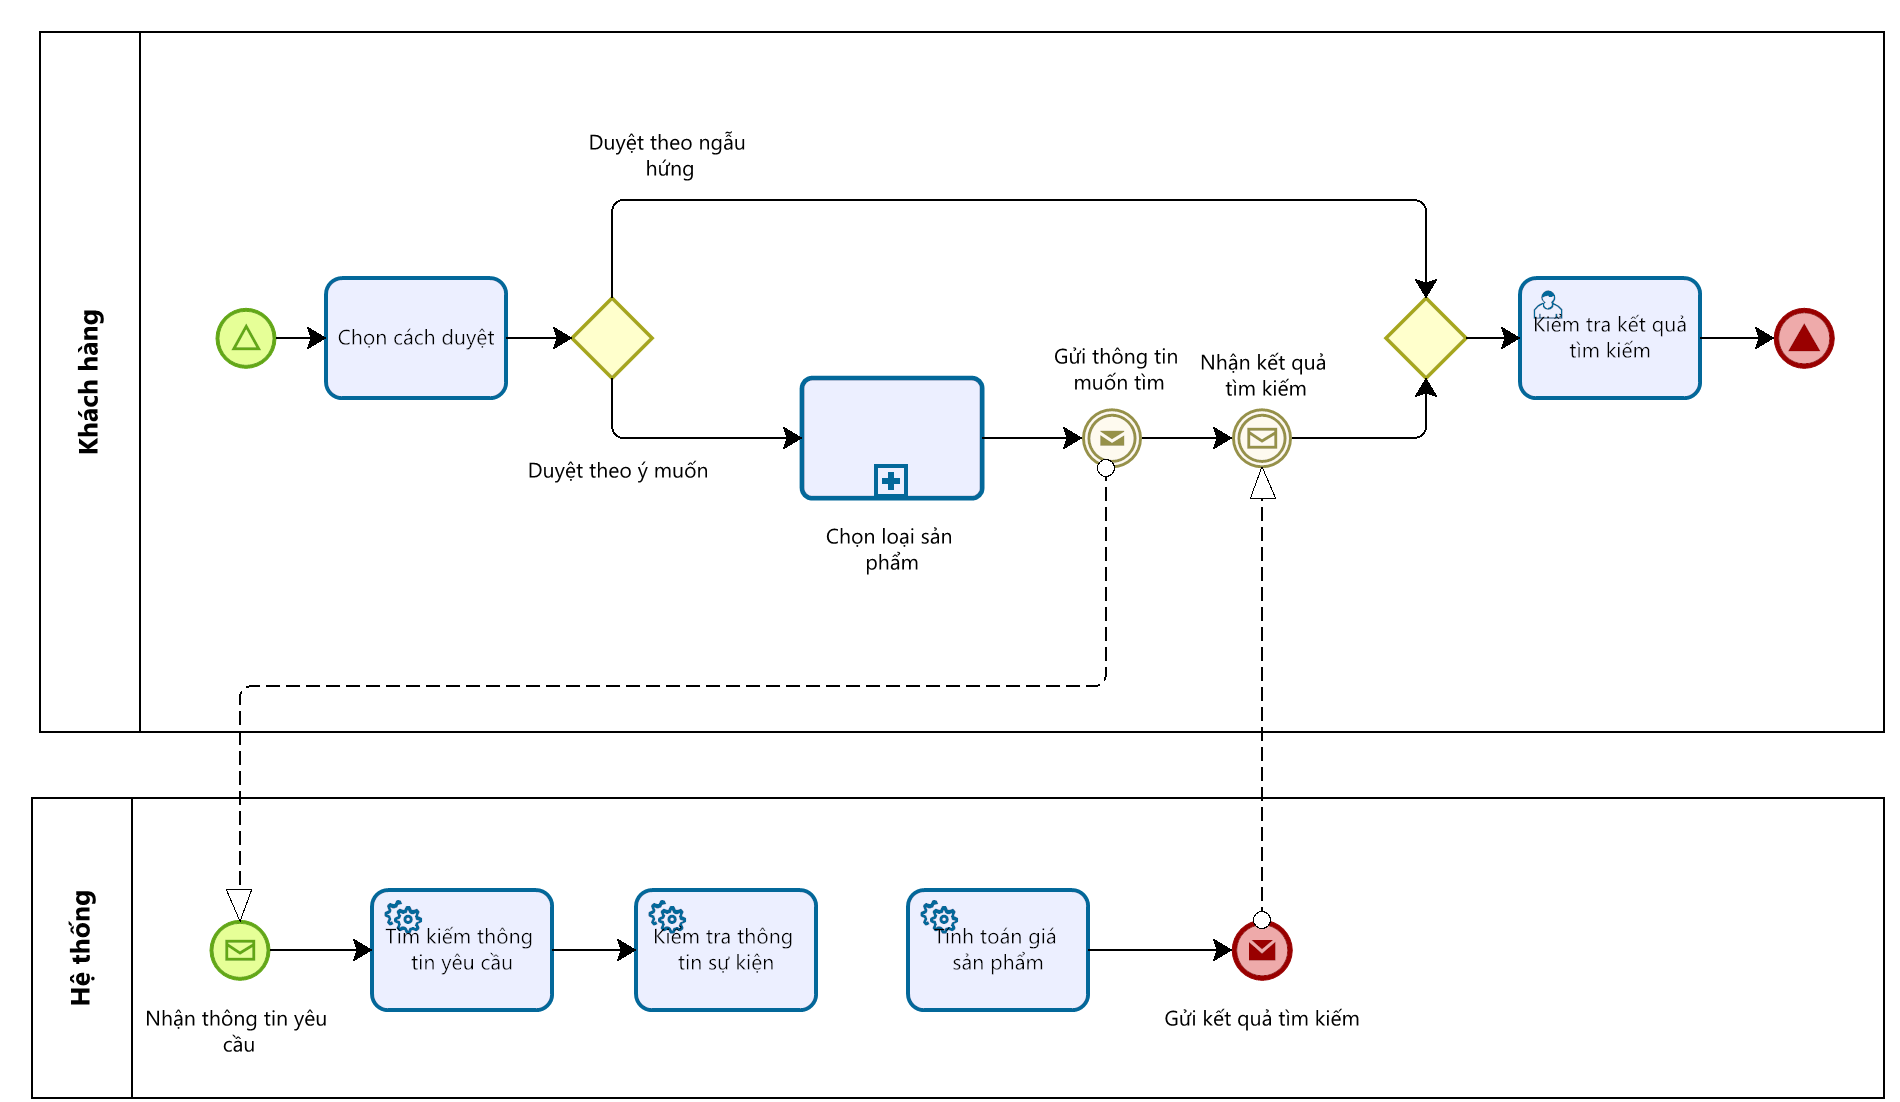
\includegraphics[width=13cm]{img/BPMN/customer_buy/customer_search_product.png}
        \label{4}
        \newline
        \caption{Lược đồ BPMN cho quy trình con tìm kiếm sản phẩm}
    \end{figure}
    \textbf{Mô tả:}
    \begin{itemize}
        \item \textbf{Chọn loại sản phầm}: Đây là 1 quy trình con chứa quy trình chọn loại sản phẩm mà người dùng muốn tình kiếm.
    \end{itemize}
    \begin{figure}[!htp]
        \centering
        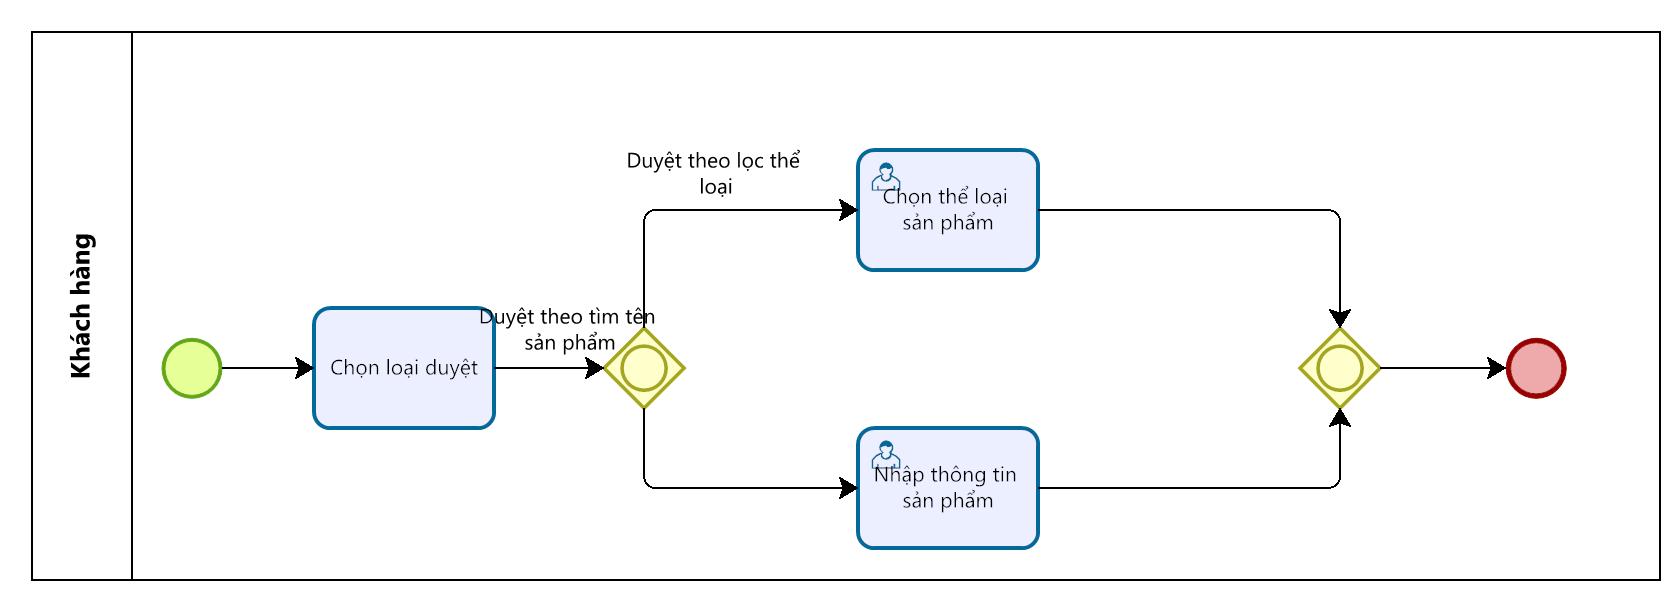
\includegraphics[width=12cm]{img/BPMN/customer_buy/customer_select_type.png}
        \label{4}
        \newline
        \caption{Lược đồ BPMN cho quy trình con chọn loại sản phẩm mà khác hàng muốn tìm}
    \end{figure}
    \begin{figure}[!htp]
        \centering
        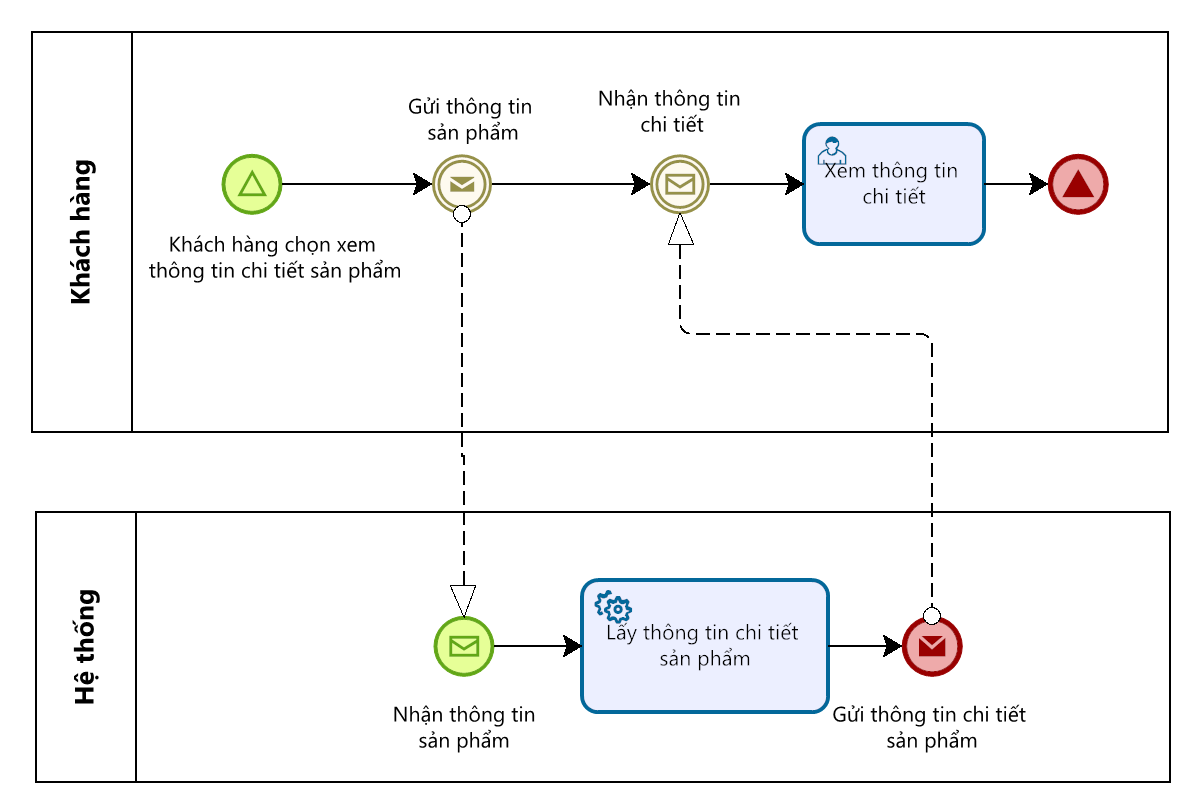
\includegraphics[width=12cm]{img/BPMN/customer_buy/customer_product_detail.png}
        \label{4}
        \newline
        \caption{Lược đồ BPMN cho quy trình xem xét thông tin chi tiết của sản phẩm}
    \end{figure}
    \begin{figure}[!htp]
        \centering
        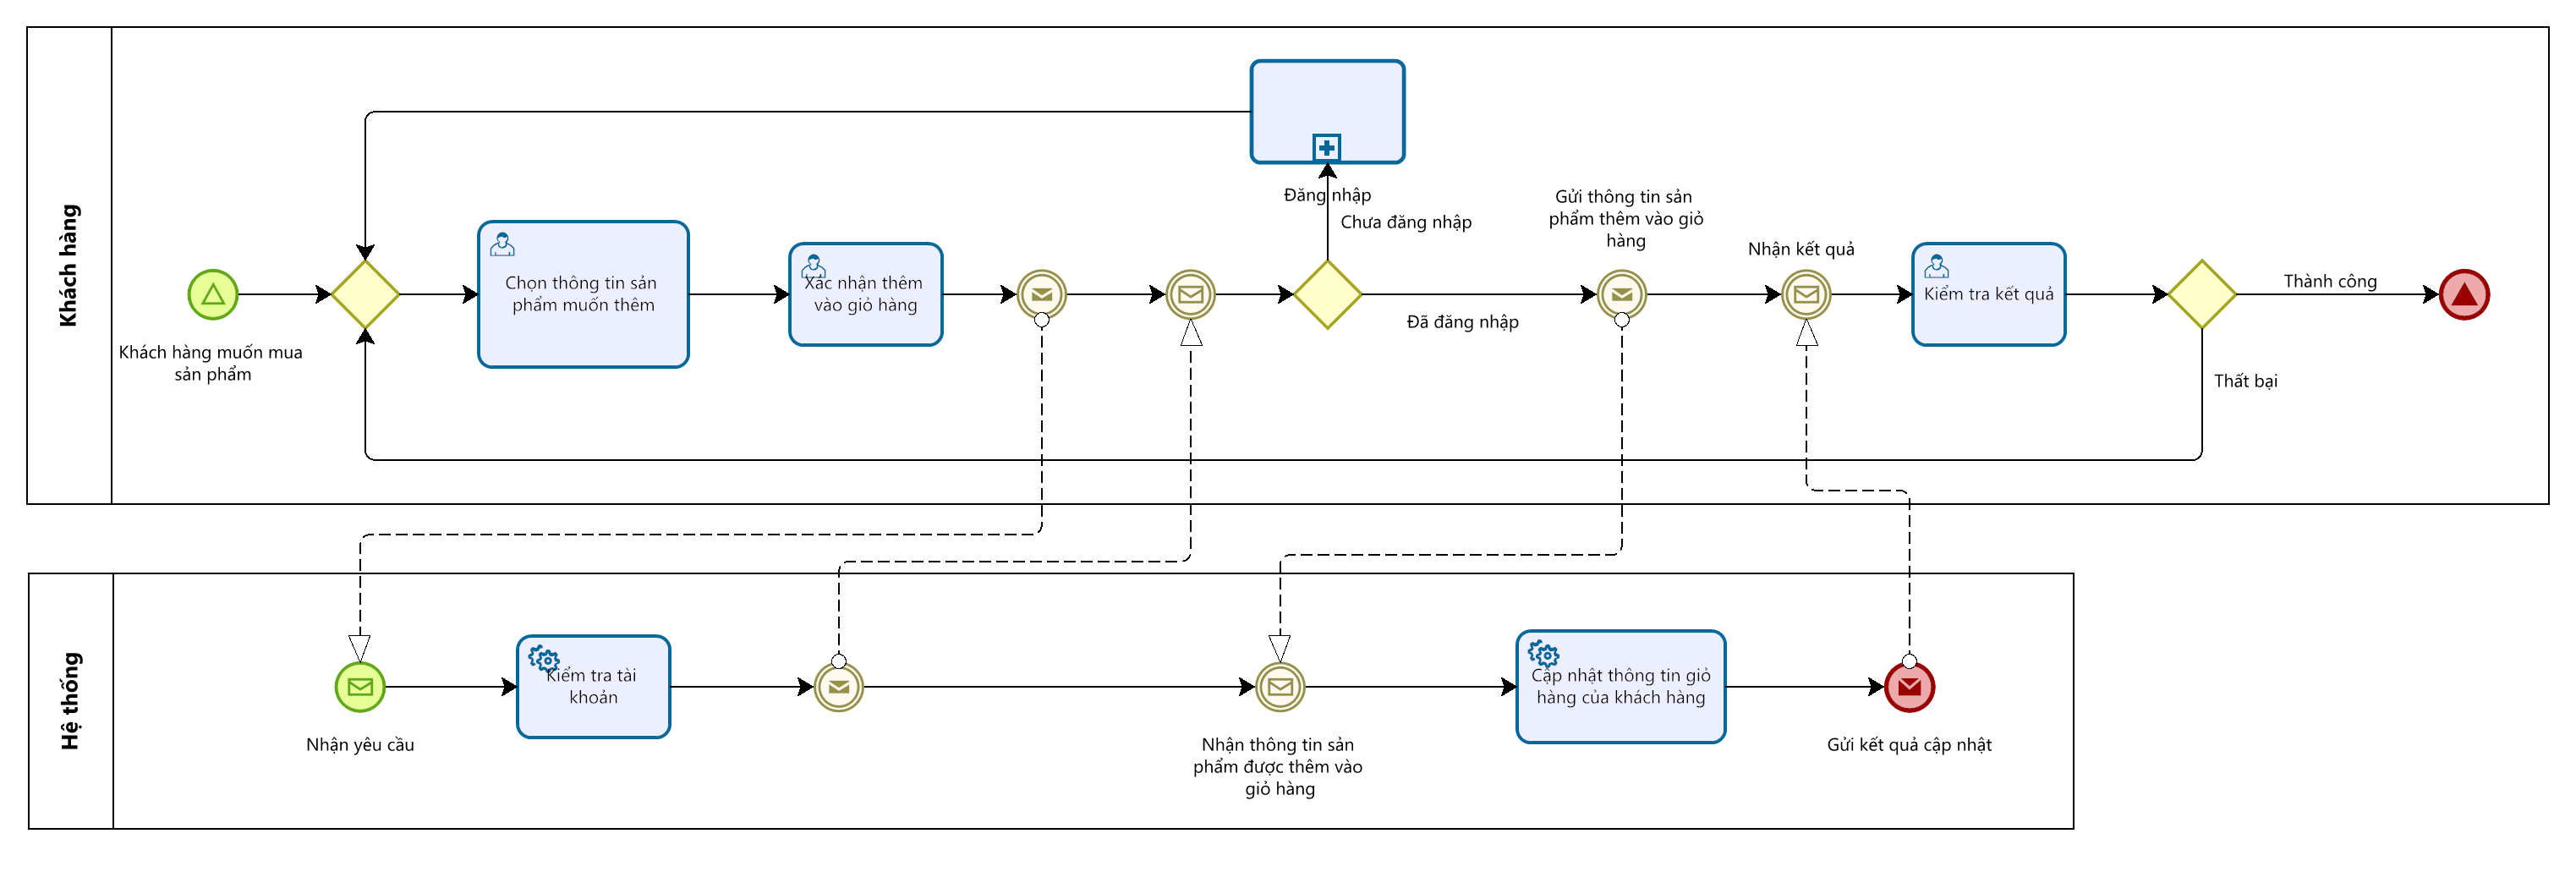
\includegraphics[width=17cm]{img/BPMN/customer_buy/customer_add_to_card.png}
        \label{4}
        \newline
        \caption{Lược đồ BPMN cho quy trình thêm sản phẩm vào giỏ hàng}
    \end{figure}  
    \begin{figure}[!htp]
        \centering
        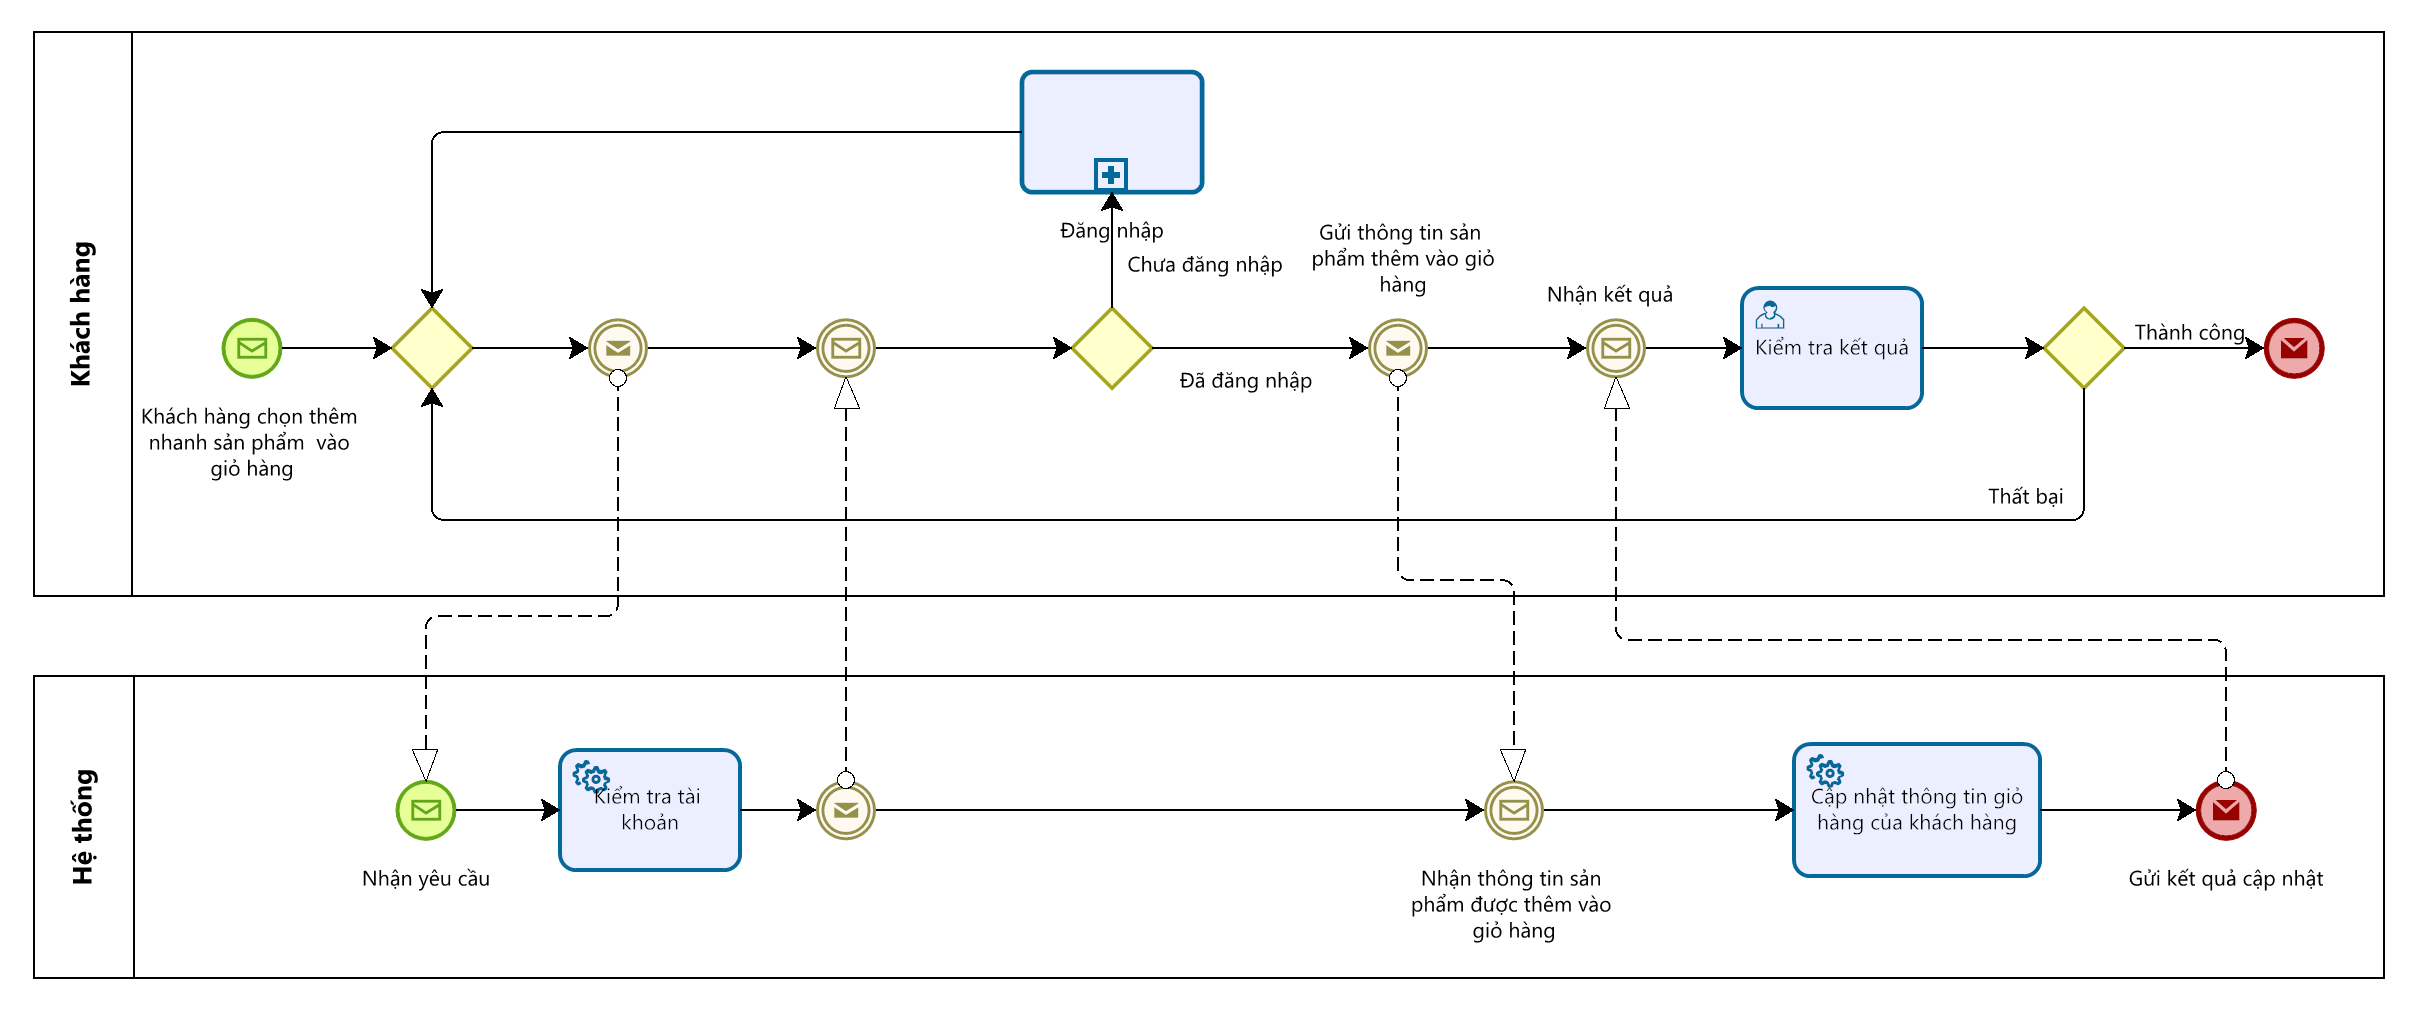
\includegraphics[width=17cm]{img/BPMN/customer_buy/customer_add_fast.png}
        \label{4}
        \newline
        \caption{Lược đồ BPMN cho quy trình thêm nhanh sản phẩm vào giỏ hàng}
    \end{figure}
    \begin{figure}[!htp]
        \centering
        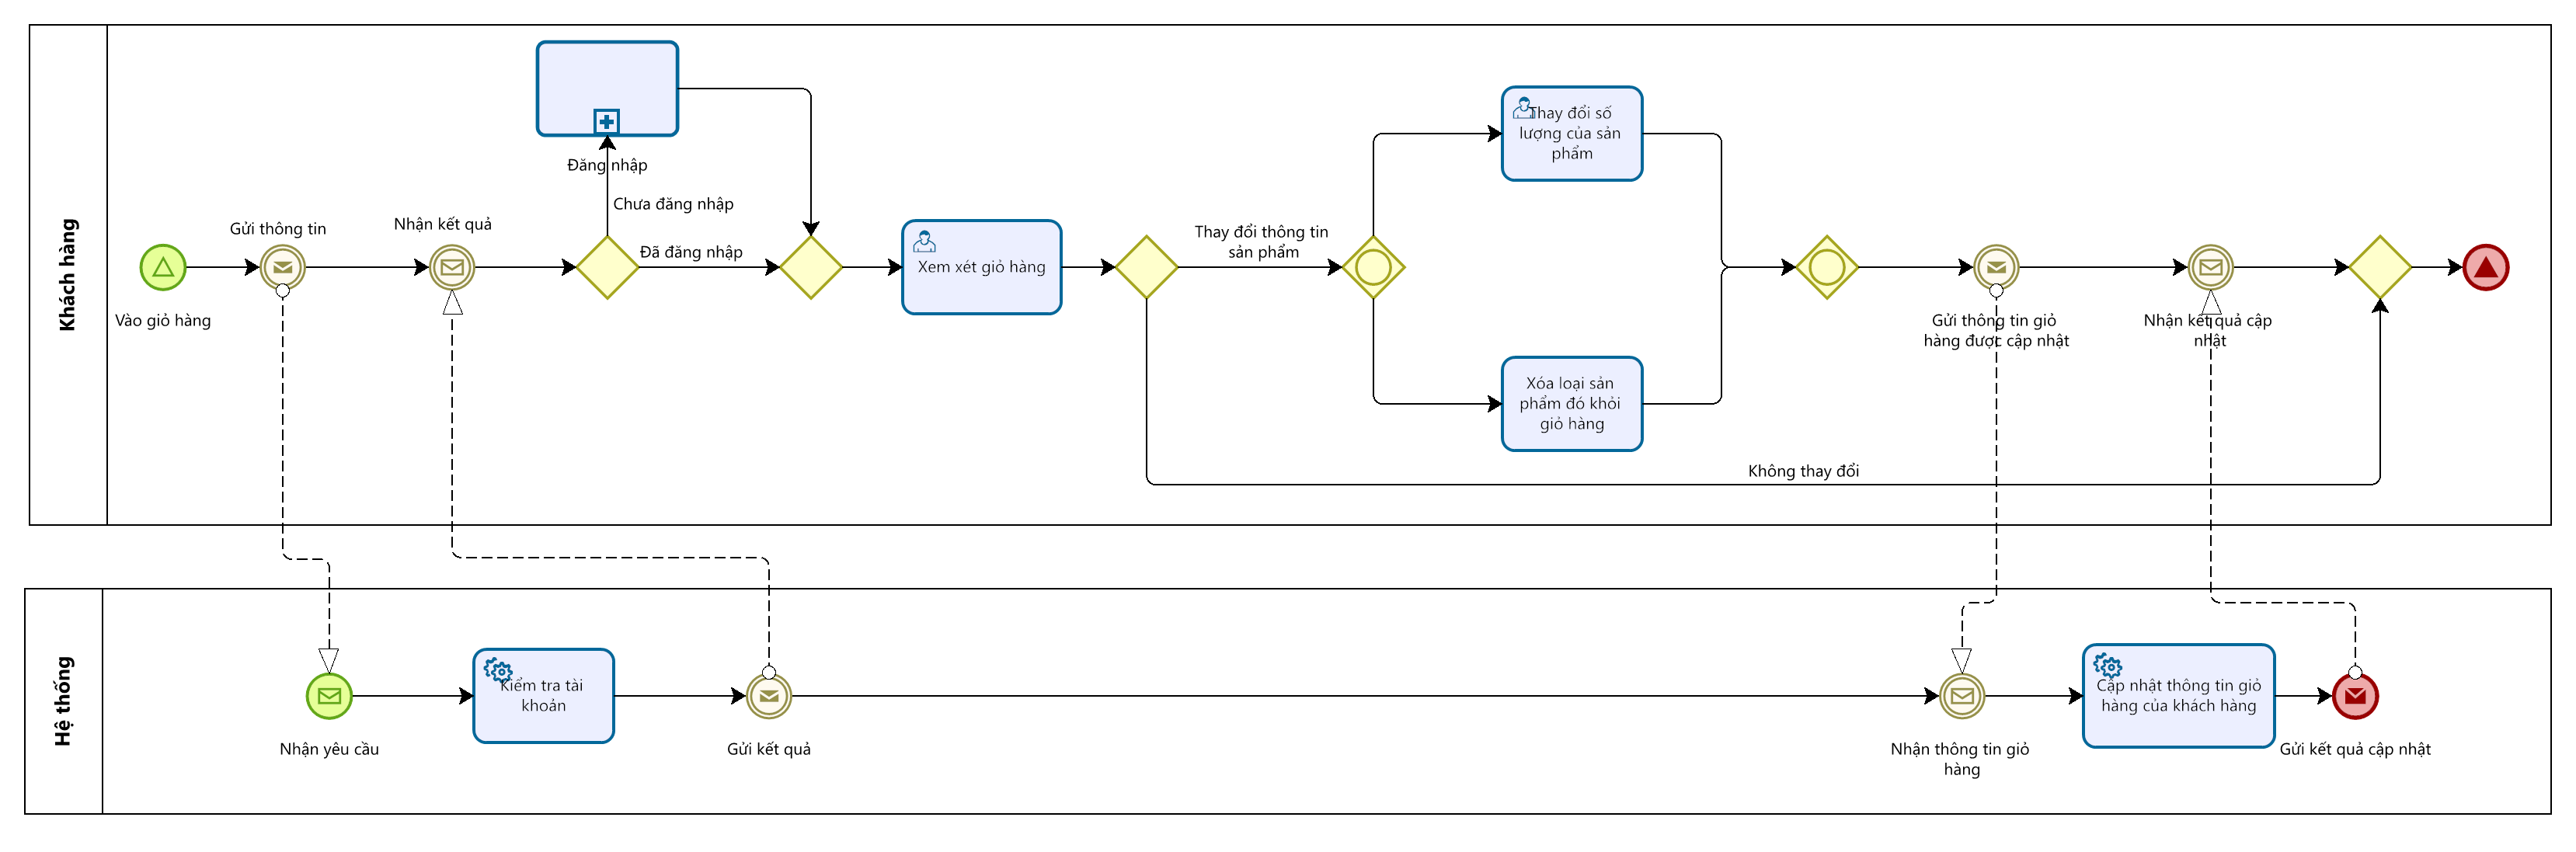
\includegraphics[width=17cm]{img/BPMN/customer_buy/customer_cart.png}
        \label{4}
        \newline
        \caption{Lược đồ BPMN cho quy trình quản lý giỏ hàng}
    \end{figure}
    \begin{figure}[!htp]
        \centering
        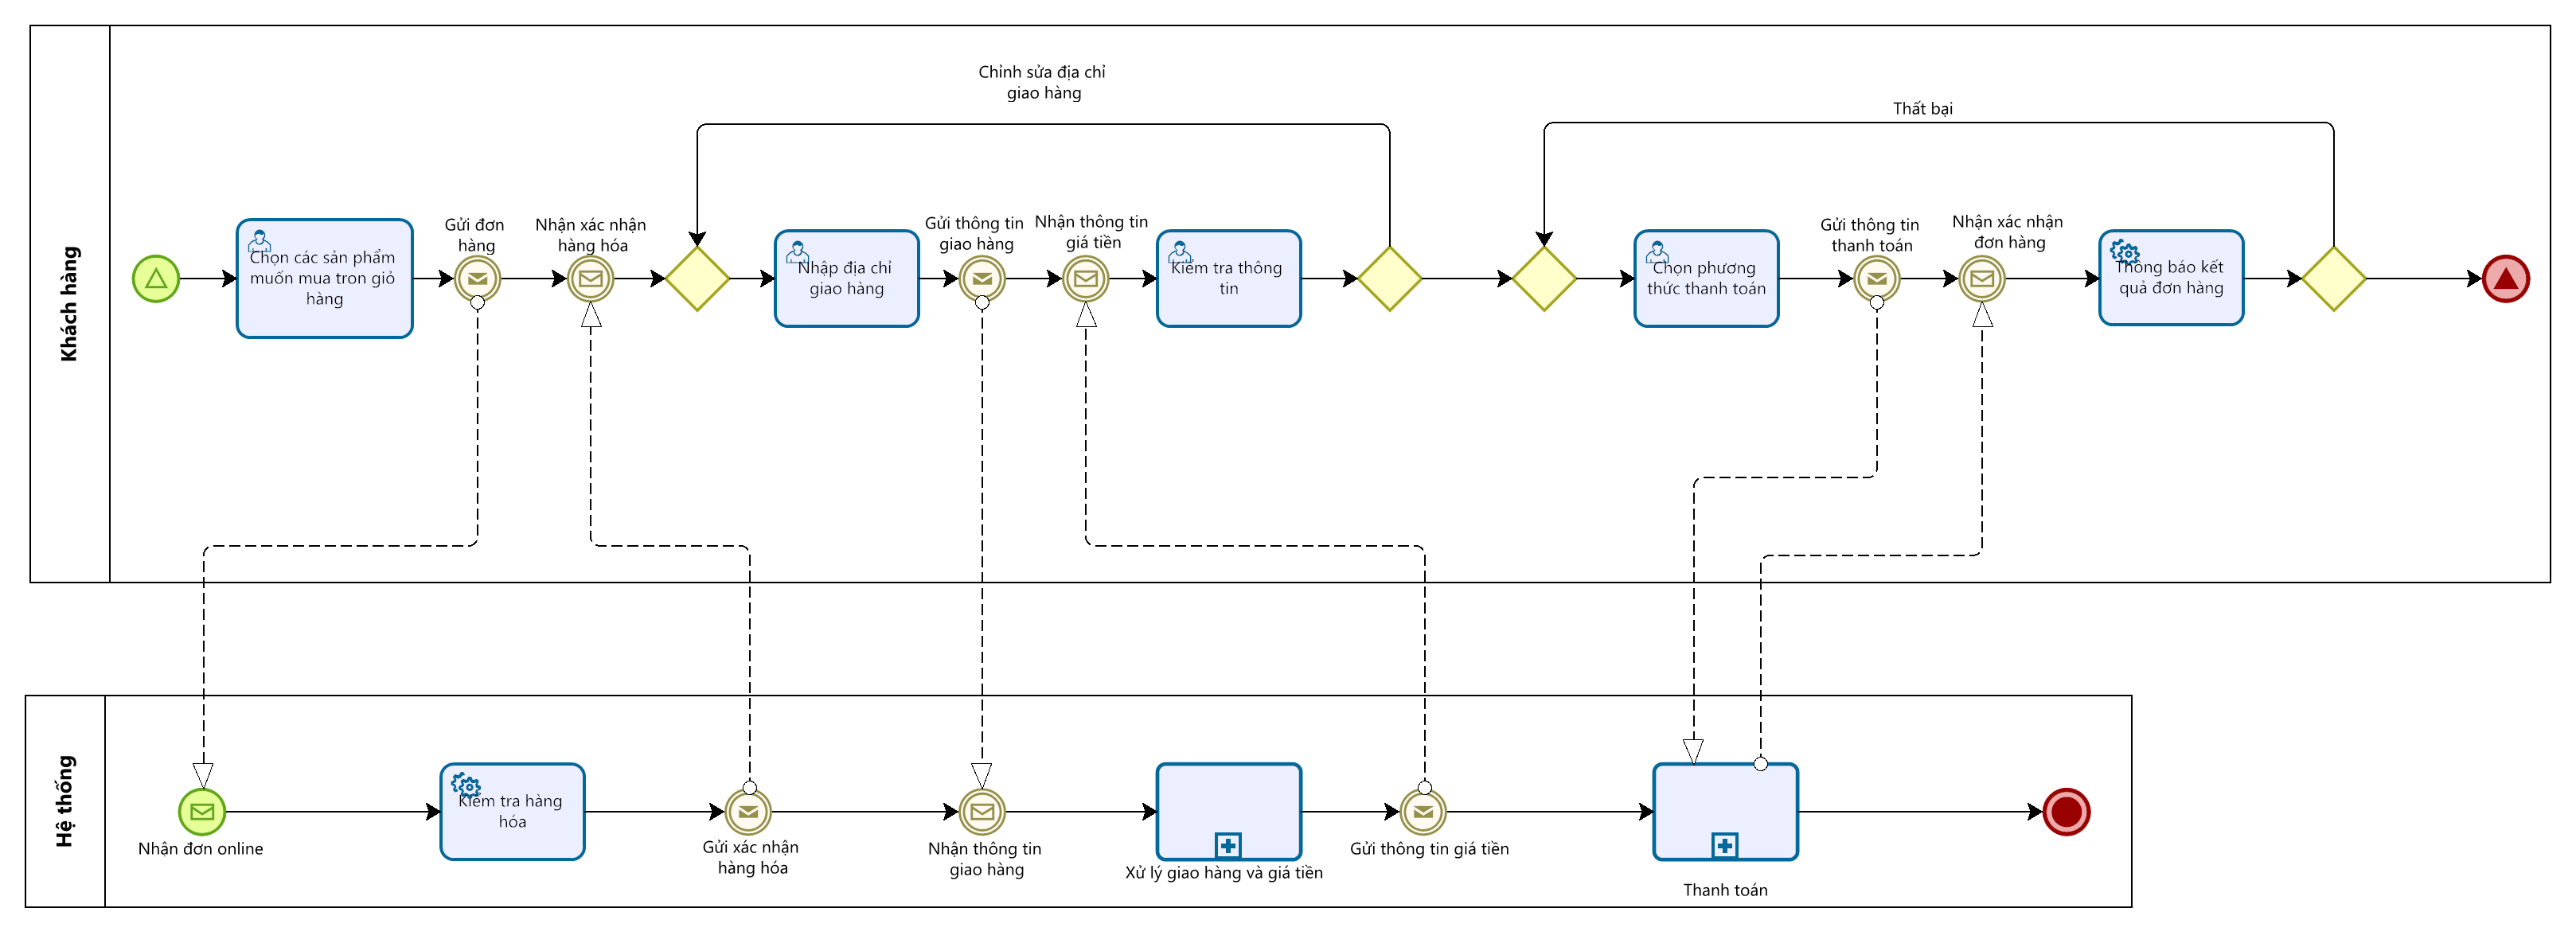
\includegraphics[width=17cm]{img/BPMN/customer_buy/customer_buy_order.png}
        \label{4}
        \newline
        \caption{Lược đồ BPMN cho quy trình mua hàng}
    \end{figure}
    \newpage
    \textbf{Mô tả:}
    \begin{itemize}
        \item \textbf{Xử lý giao hàng và giá tiền}: Đây là 1 quy trình con chứa quy trình con xử lý về dịch vụ giao hàng cho đơn hàng và tính toán tất cả các chi phí.
        \item \textbf{Thanh toán}: Đây là 1 quy trình con chứa quy trình thanh toán đơn hàng của khách hàng.
    \end{itemize}
    \begin{figure}[!htp]
        \centering
        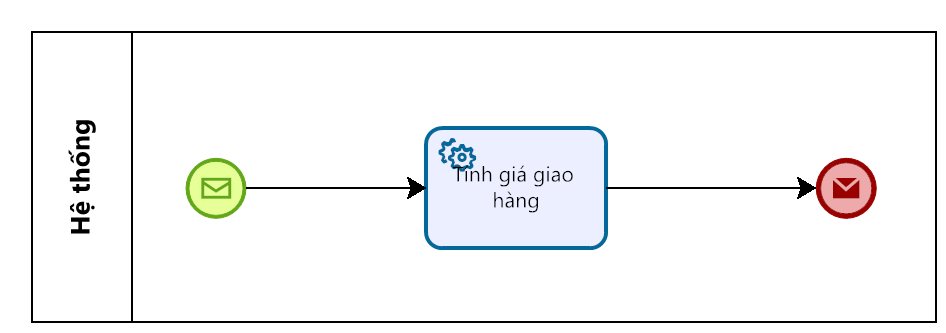
\includegraphics[width=5in]{img/BPMN/customer_buy/customer_calc_fee.png}
        \label{4}
        \newline
        \caption{Lược đồ BPMN cho quy trình tính toán chi phí đơn hàng}
    \end{figure}
    \begin{figure}[!htp]
        \centering
        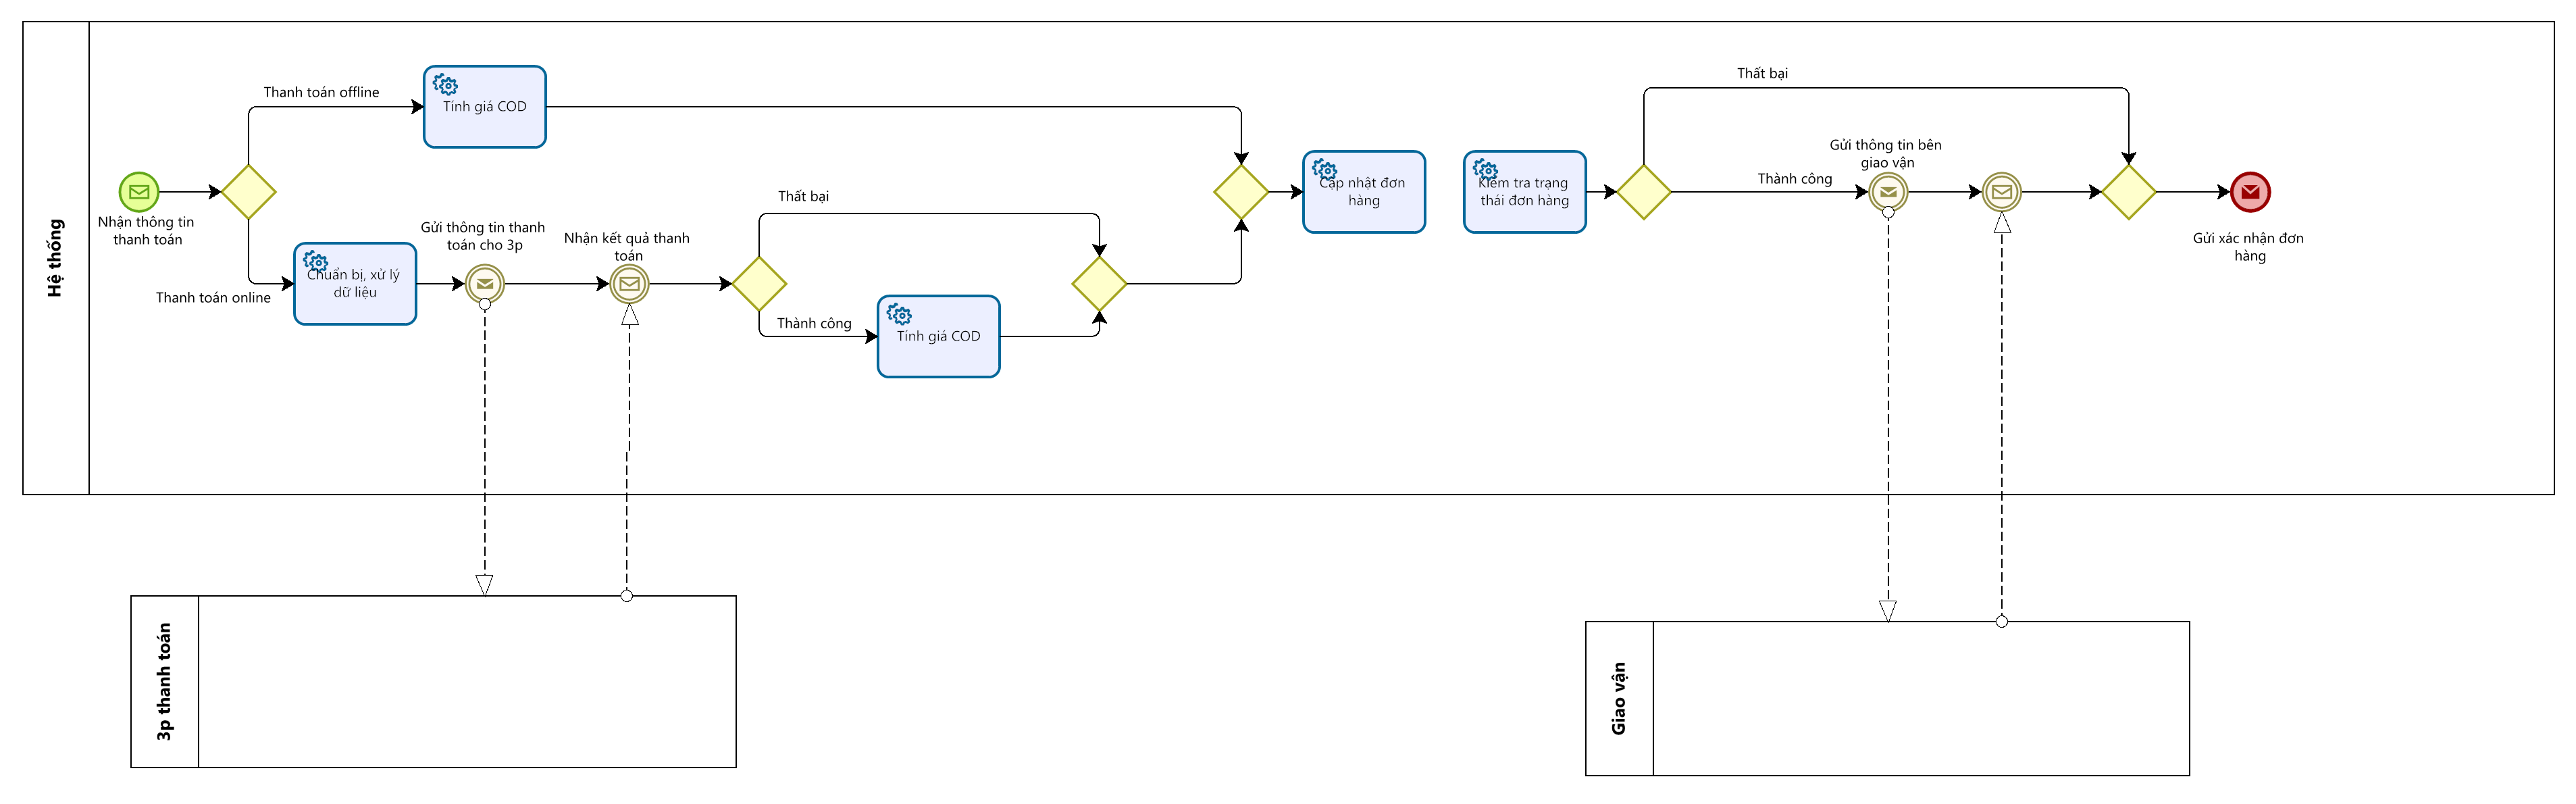
\includegraphics[width=17cm]{img/BPMN/customer_buy/customer_payment.png}
        \label{4}
        \newline
        \caption{Lược đồ BPMN cho quy trình thanh toán đơn hàng}
    \end{figure}

\subsection{Khách hàng mua hàng trực tiếp}
\begin{figure}[!htp]
    \centering
    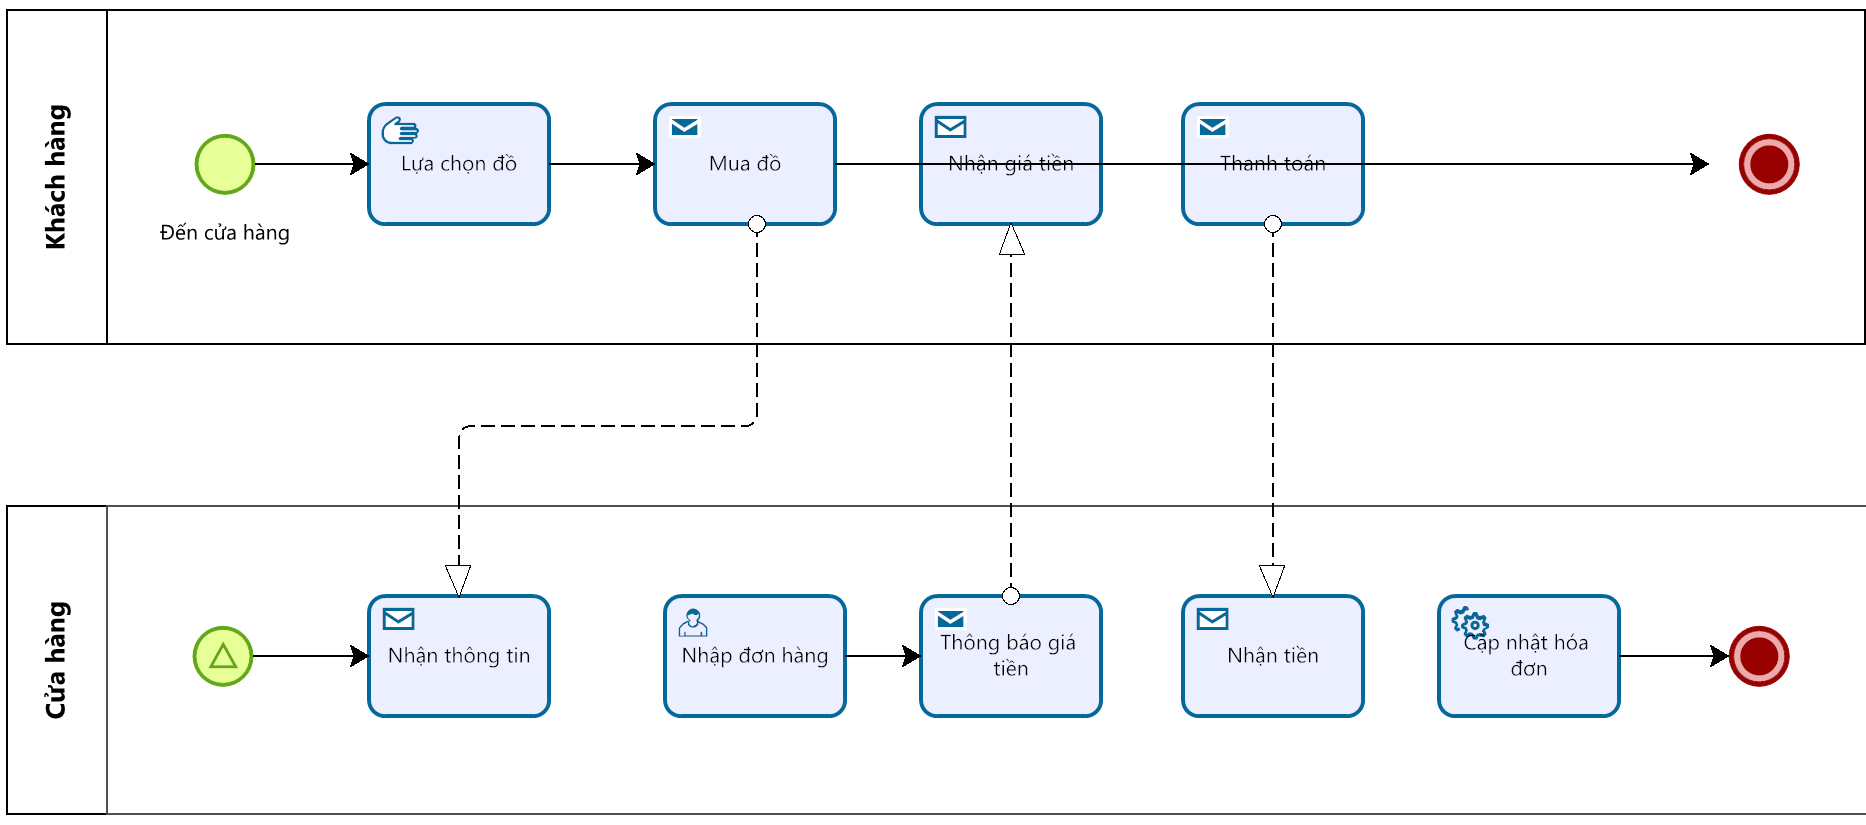
\includegraphics[width=14cm]{img/BPMN/Hien/Customer_buyOffline.png}
    \newline
    \caption{Lược đồ BPMN cho quy trình khách hàng mua hàng trực tiếp}
\end{figure}

\subsection{Đăng nhập}
\begin{figure}[!htp]
    \centering
    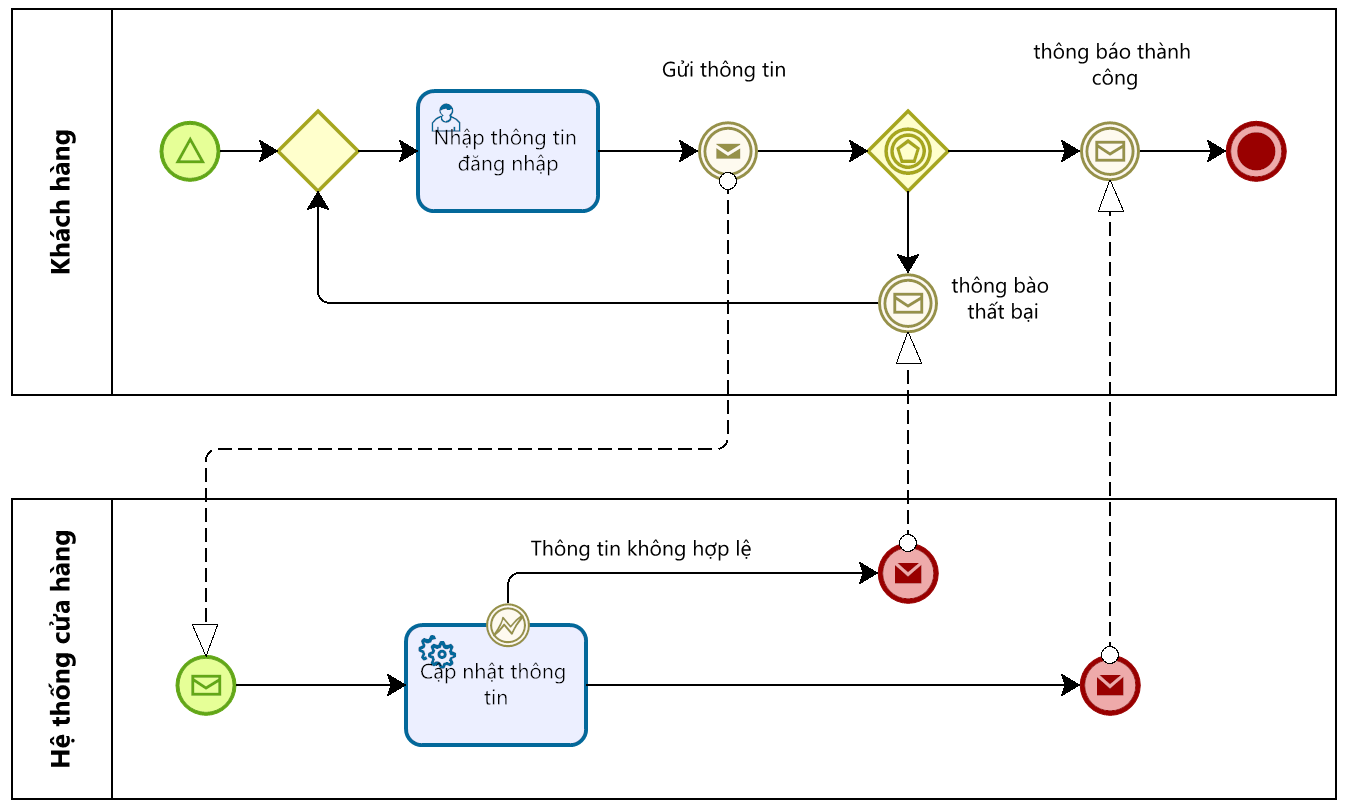
\includegraphics[width=14cm]{img/BPMN/Hien/Customer_login.png}
    \newline
    \caption{Lược đồ BPMN cho quy trình đăng nhập}
\end{figure}

\subsection{Đăng ký tài khoản}
\begin{figure}[!htp]
    \centering
    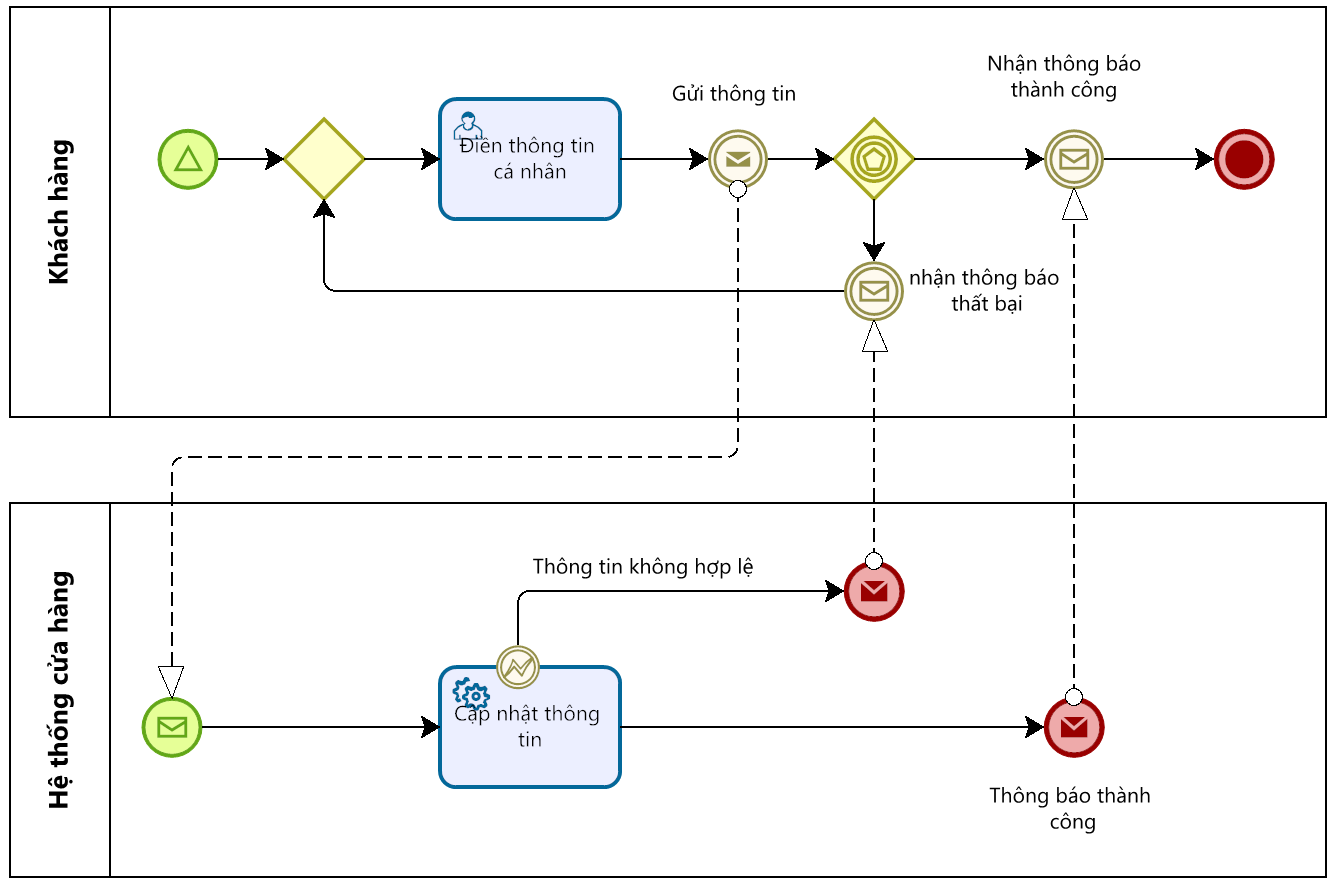
\includegraphics[width=14cm]{img/BPMN/Hien/Customer_register.png}
    \newline
    \caption{Lược đồ BPMN cho quy trình đăng ký tài khoản mới}
\end{figure}


\subsection{Làm mới mật khẩu}
\begin{figure}[!htp]
    \centering
    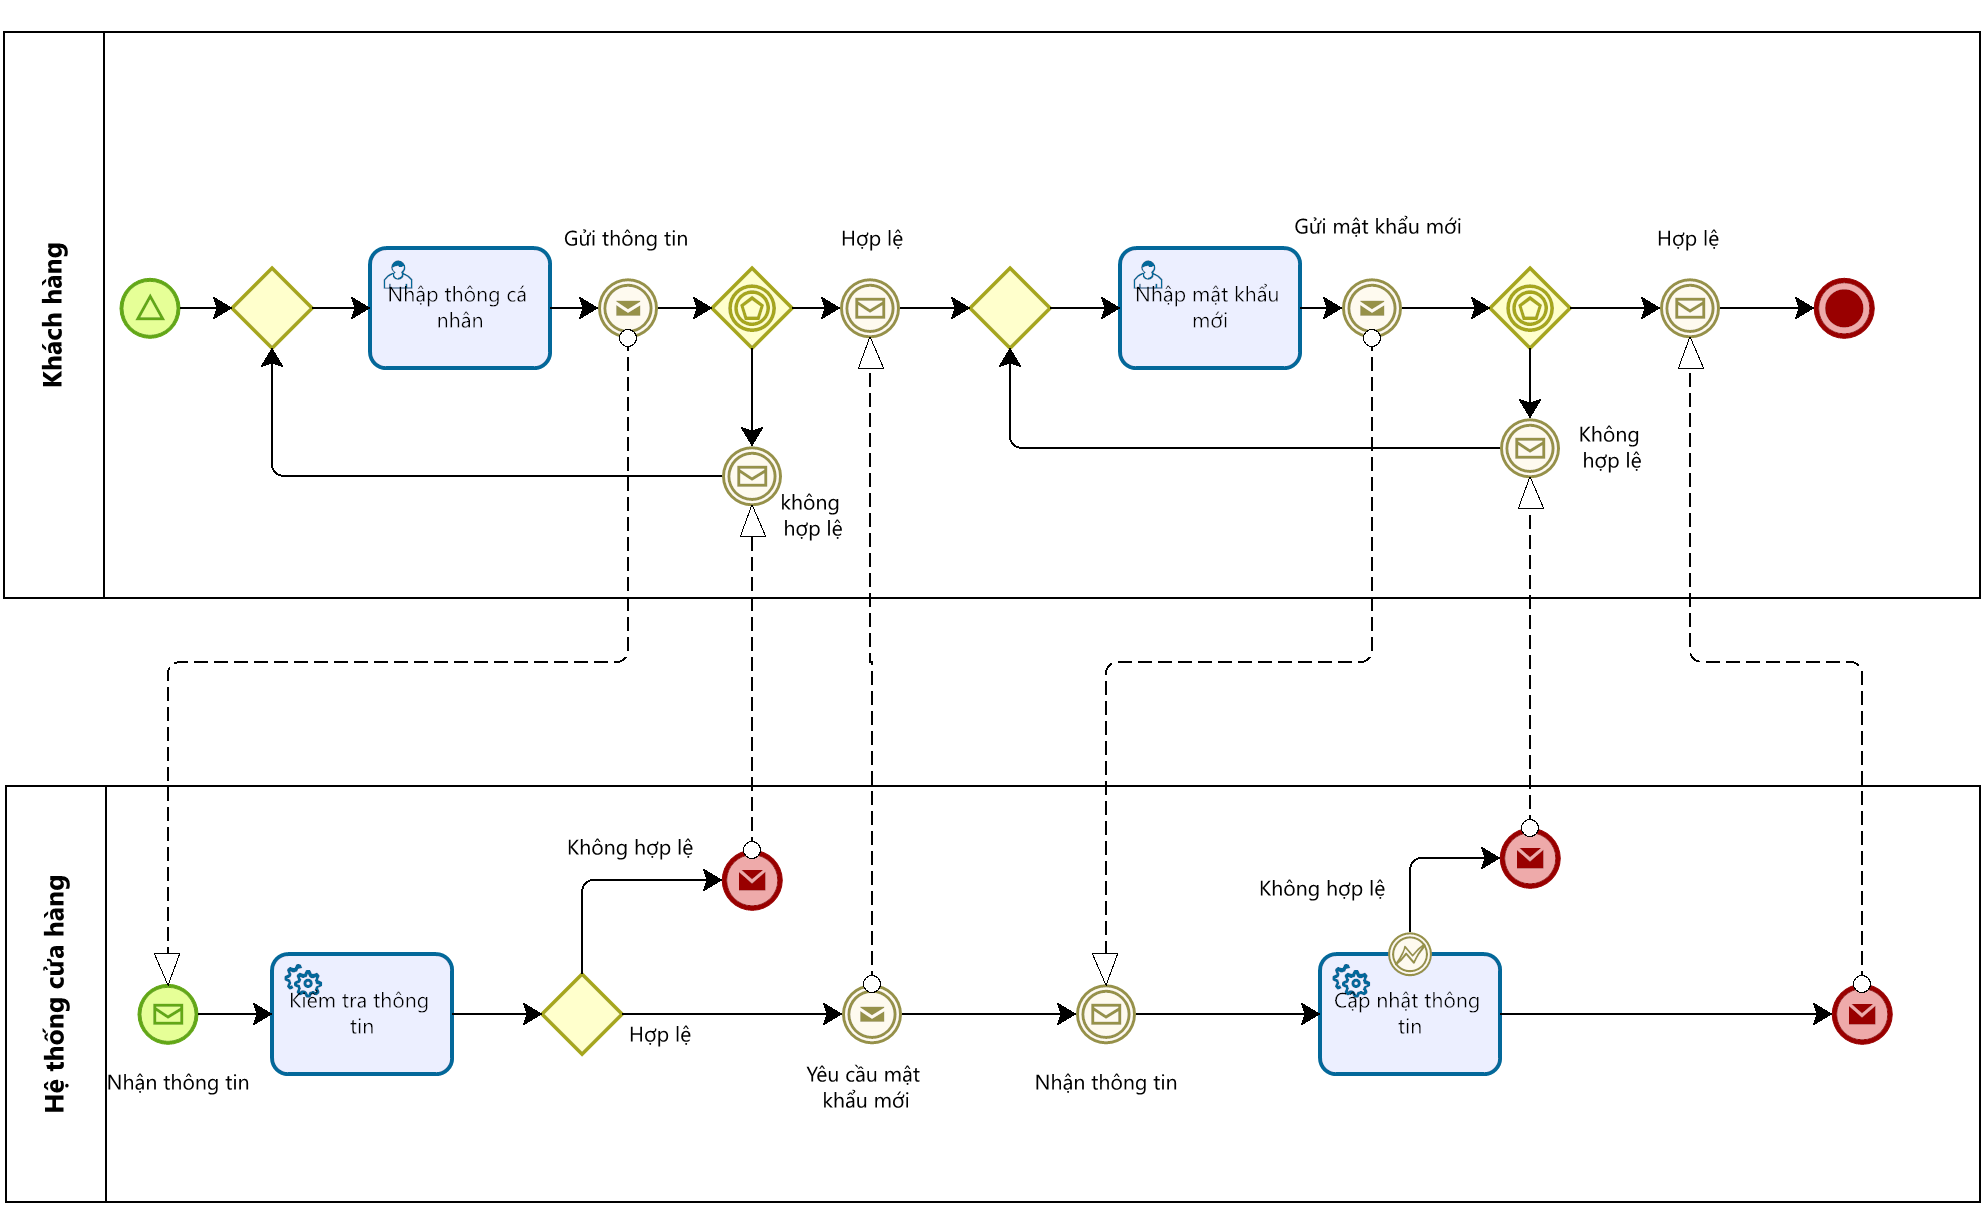
\includegraphics[width=14cm]{img/BPMN/Hien/Customer_resetPassword.png}
    \newline
    \caption{Lược đồ BPMN cho quy trình làm mới mật khẩu}
\end{figure}



\subsection{Quản lý chi nhánh}
\begin{figure}[!htp]
    \centering
    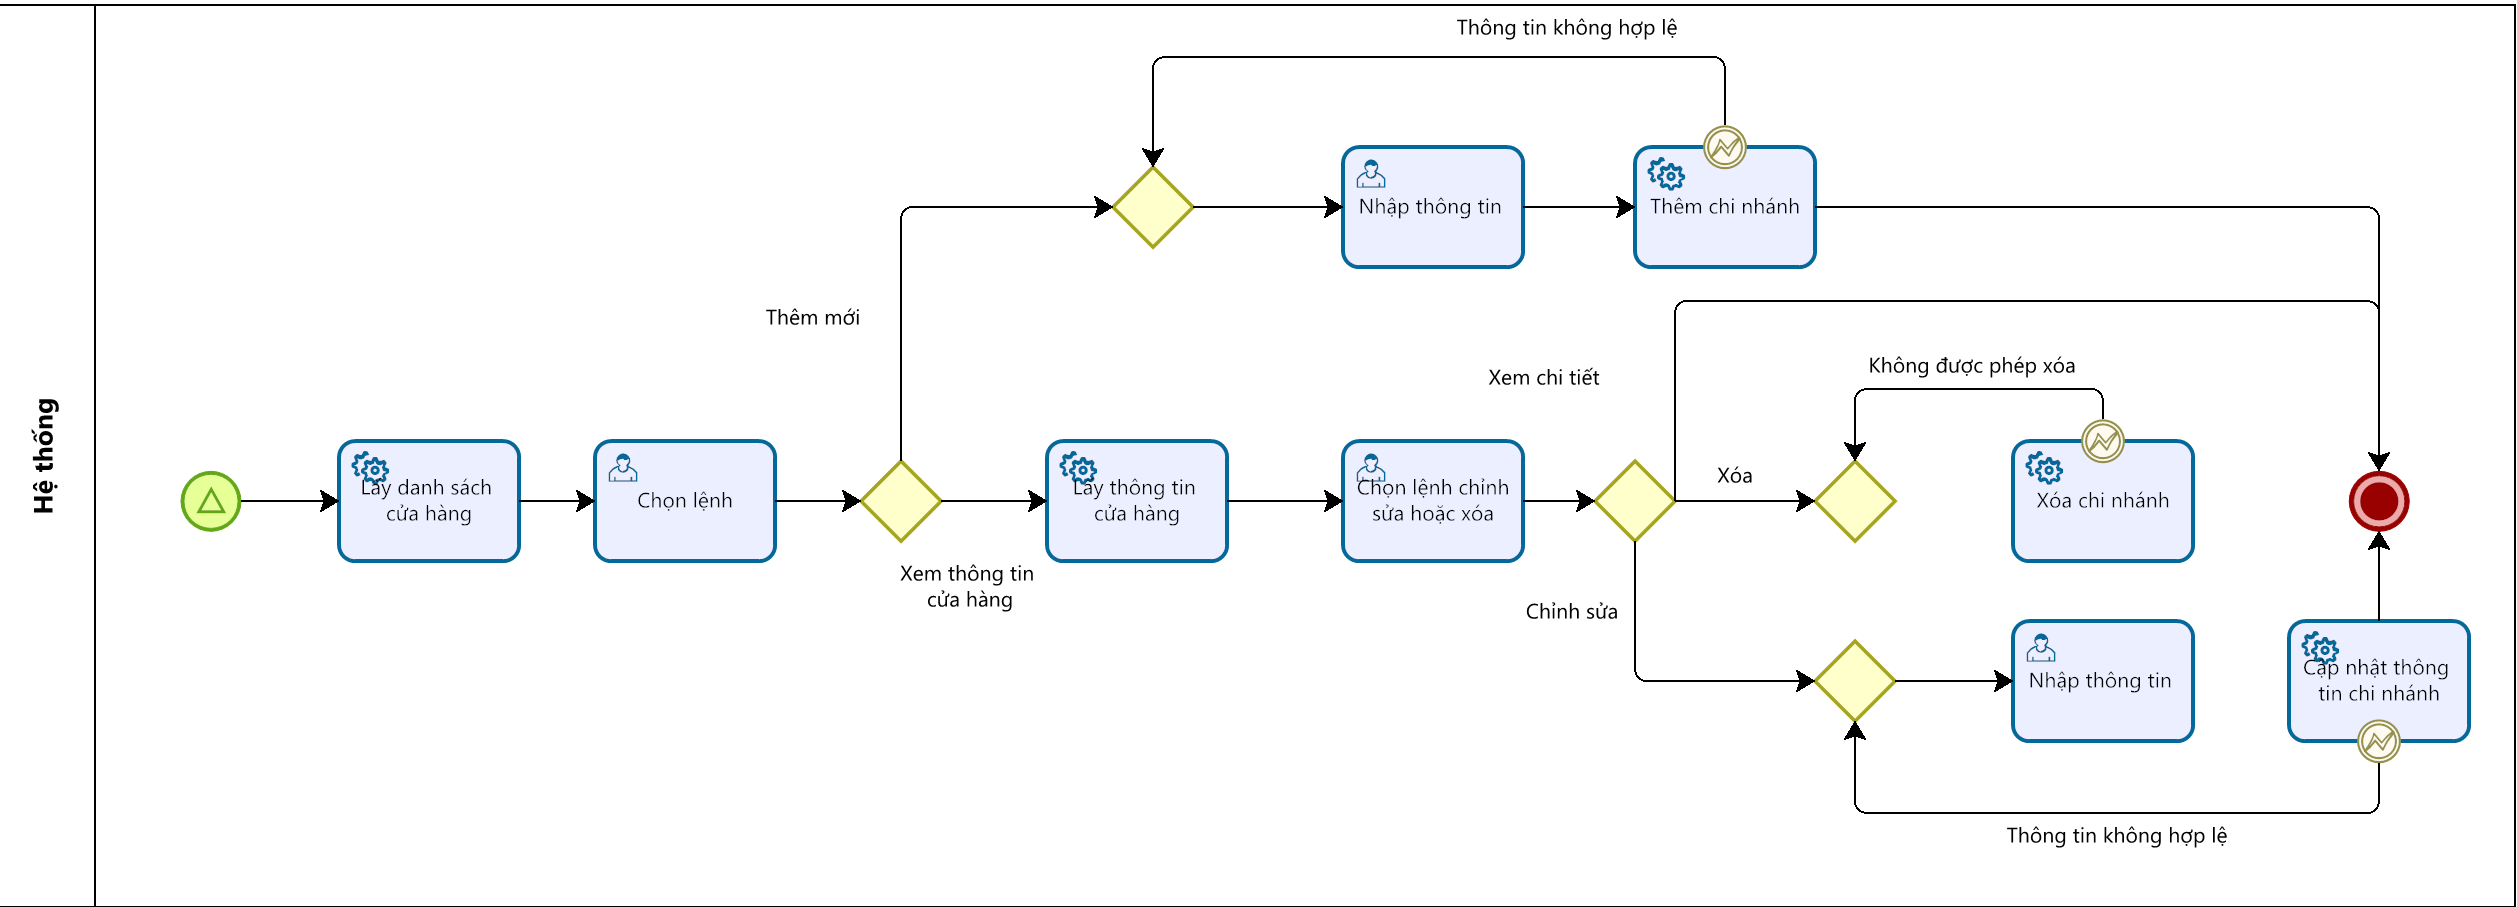
\includegraphics[width=14cm]{img/BPMN/Hien/Branch_management.png}
    \newline
    \caption{Lược đồ BPMN cho quy trình quản lý chi nhánh}
\end{figure}


\subsection{Quản lý nhân viên}
\begin{figure}[!htp]
    \centering
    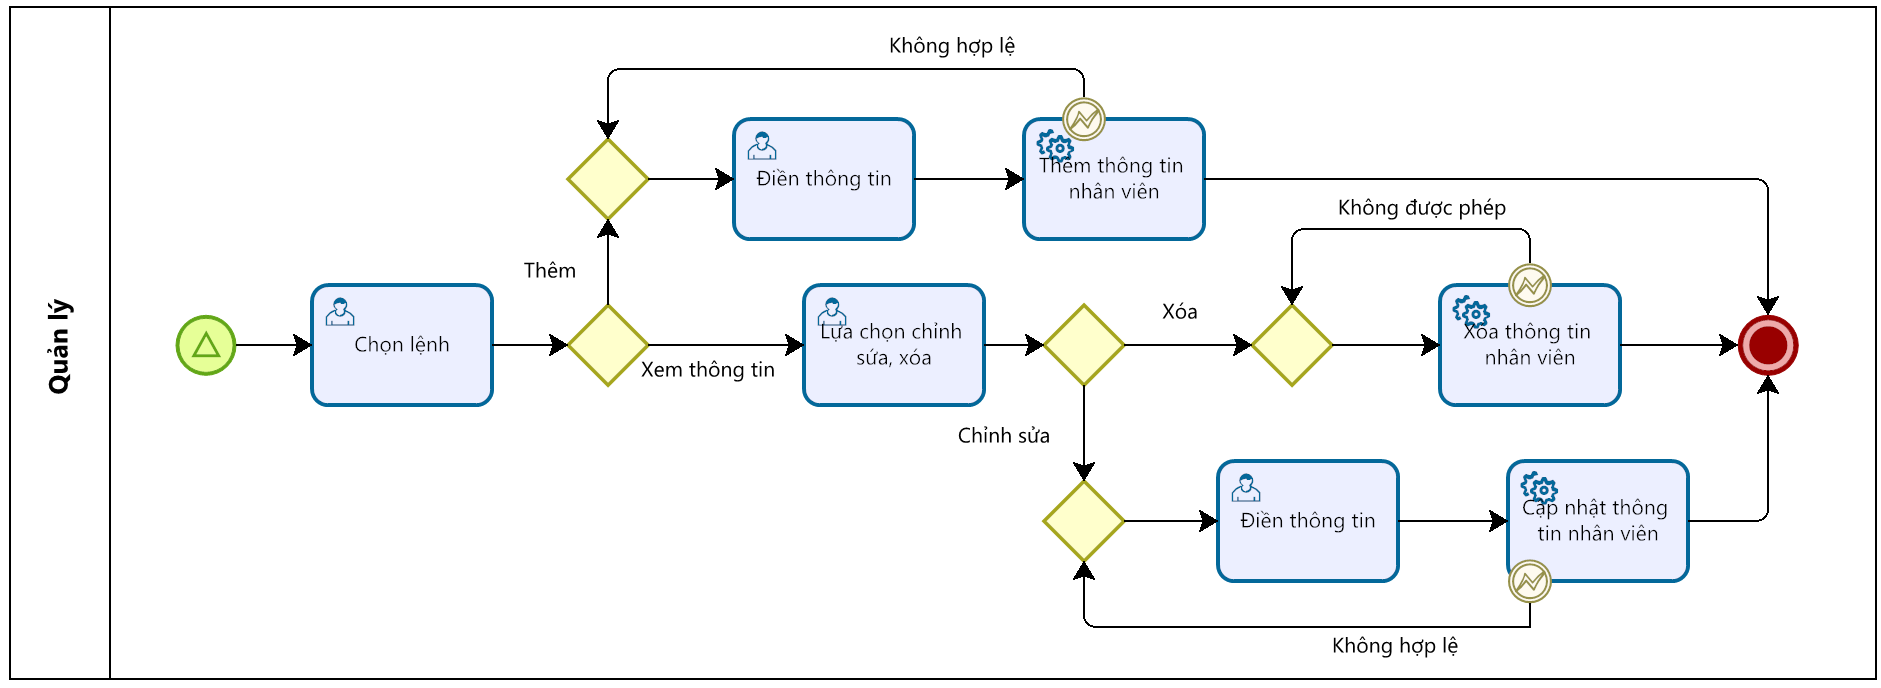
\includegraphics[width=14cm]{img/BPMN/Hien/Employee_Management.png}
    \newline
    \caption{Lược đồ BPMN cho quy trình quản lý nhân viên}
\end{figure}

\subsubsection*{Tạo yêu cầu thêm, xóa nhân viên}
\begin{figure}[!htp]
    \centering
    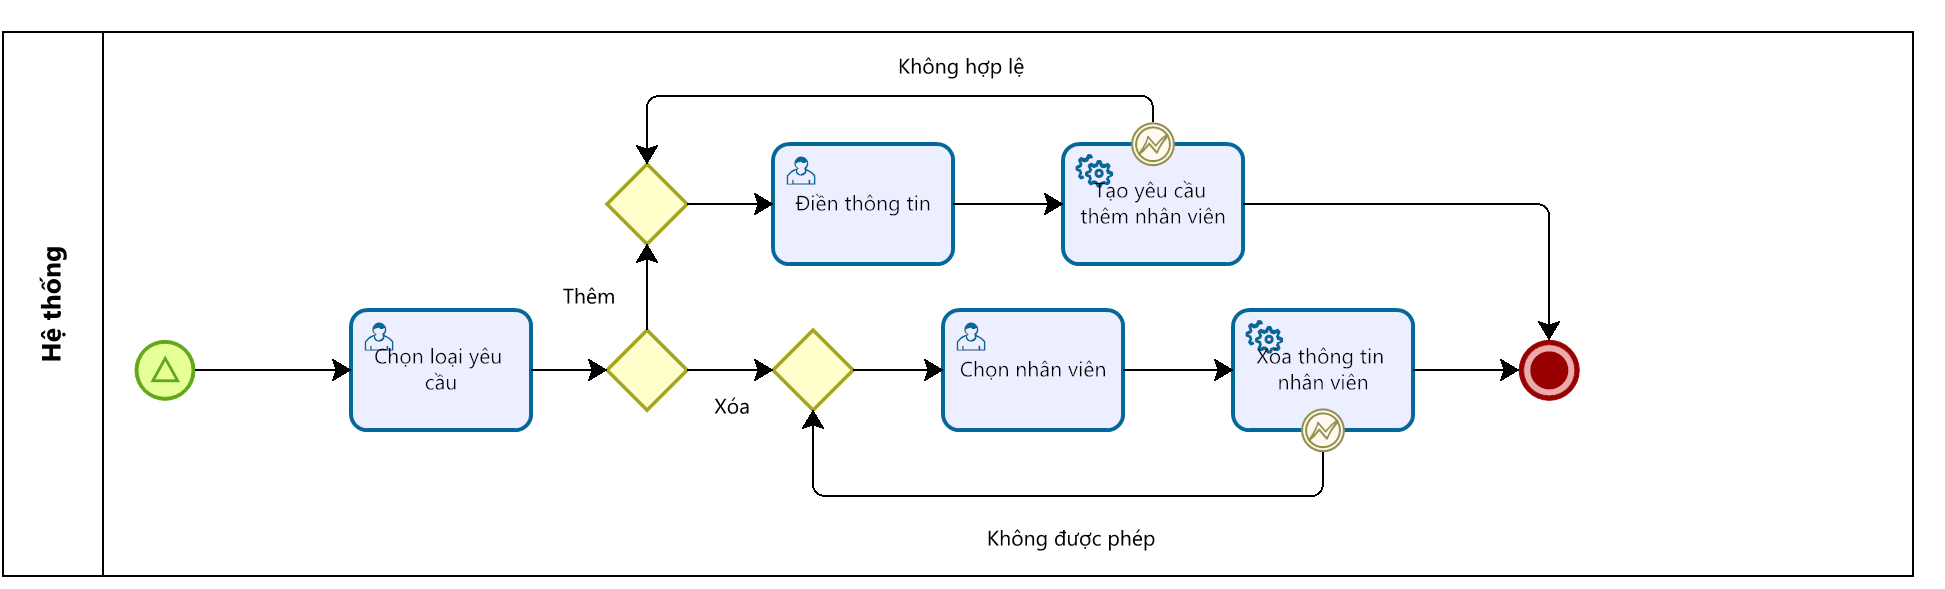
\includegraphics[width=14cm]{img/BPMN/Hien/Employee_request.png}
    \newline
    \caption{Lược đồ BPMN cho quy trình quản lý nhân viên}
\end{figure}

